% Created 2021-02-11 Thu 15:13
% Intended LaTeX compiler: pdflatex
\documentclass[11pt]{article}
\usepackage[hyphens]{url}
\usepackage{float}
\usepackage[utf8]{inputenc}
\usepackage[T1]{fontenc}
\usepackage{graphicx}
\usepackage{grffile}
\usepackage{longtable}
\usepackage{wrapfig}
\usepackage{rotating}
\usepackage[normalem]{ulem}
\usepackage{amsmath}
\usepackage{textcomp}
\usepackage{amssymb}
\usepackage{capt-of}
\usepackage{hyperref}
\author{Tigany Zarrouk\thanks{tigany.zarrouk@kcl.ac.uk}}
\date{09.04.2019}
\title{Atomic scale stress corrosion cracking of Ti alloys.}
\hypersetup{
 pdfauthor={Tigany Zarrouk},
 pdftitle={Atomic scale stress corrosion cracking of Ti alloys.},
 pdfkeywords={},
 pdfsubject={},
 pdfcreator={Emacs 27.1 (Org mode 9.4.4)}, 
 pdflang={English}}
\begin{document}

\maketitle


\section*{Motivation}
\label{sec:org792ceb1}
\begin{itemize}
\item Titanium alloys are used in highly demanding circumstances.
\item Brittle oxide layer can crack.
\item Solutes affect dislocation mobility, causing hardening.
\item Interaction between oxygen and dislocation cores is not clear.
\item Need for atomistic modelling.
\item Exploration of Ti/oxide scale interface will give insights into oxygen
diffusion, oxygen induces brittleness and stress corrosion cracking in Ti
alloys.
\end{itemize}
\begin{NOTES}
\begin{itemize}
\item Corrosion resistance, high strength to weight ratio.
\item Ti is used in commercial jet airliners
\end{itemize}
\end{NOTES}


\section*{Quantum Methods}
\label{sec:orgc1f9e9c}
\begin{itemize}
\item Density Functional Theory is not feasible.
\item System size is limited due to computational cost.
\item Boundaries of cell affect relaxation of core more.
\item Semi-empirical method is more computationally efficient.
\end{itemize}

\subsection*{Tight Binding}
\label{sec:org8cd49e8}


\begin{itemize}
\item Tight binding is an approximation to DFT.
\item Overlaps between atomic orbitals are key parameters.
\item Parameters can be fitted to experimental data
\item \(\mathcal{O}(N^3)\), but much smaller prefactor compared to DFT.
\end{itemize}

\subsection*{BOP}
\label{sec:org3a1ab53}

\begin{itemize}
\item BOP is a faster but less accurate \(\mathcal{O}(N)\) method of interatomic
force calculation within tight-binding.
\item One builds a local density of states from moments, giving detailed
electronic structure information.
\end{itemize}


\subsection*{Embedding}
\label{sec:orgba9c5a8}

\begin{itemize}
\item Idea is to combine speed of BOP (\(\mathcal{O}(N)\)) with accuracy of
tight-binding \(\mathcal{O}(N^3)\).
\item Increasing the number of atoms gives freedom to:
\begin{itemize}
\item Investigate isolated dislocations.
\item Include solutes at more realistic concentrations.
\item Simulate interfaces near a surface (e.g. TiO\(_2\) and
bulk Ti)
\end{itemize}
\end{itemize}
\begin{NOTES}
Invariance theorem with green's function approaches. So good with boundary
conditions. 
\end{NOTES}


\section*{Parameter Optimisation}
\label{sec:org4a1103a}
\begin{itemize}
\item Parameter set for TB model optimised by two evolutionary algorithms: genetic
and particle swarm.
\item More optimisation necessary. Interim model used for simulations.
\item Similar tests can improve the optimisation procedure such
that parameters are not overfit to training data.
\end{itemize}

\subsection*{Results of optimisation.}
\label{sec:org9b1b452}
\begin{center}
\begin{tabular}{lrrr}
\hline
Quantity & TB & BOP & target\\
\hline
\(a_{\alpha}\)              [bohr] & 5.42 & 5.20 & 5.57\\
\(c_{\alpha}\)              [bohr] & 8.72 & 9.15 & 8.85\\
\(C_{11}\)                  [GPa ] & 221.8 & 218.1 & 176.1\\
\(C_{33}\)                  [GPa ] & 194.2 & 263.4 & 190.5\\
\(C_{44}\)                  [GPa ] & 58.6 & -8.5 & 50.8\\
\(C_{12}\)                  [GPa ] & 71.4 & 93.6 & 86.9\\
\(C_{13}\)                  [GPa ] & 60.0 & 54.4 & 68.3\\
\(a_{\omega}\)              [bohr] & 8.50 & 8.34 & 8.73\\
\(c_{\omega}\)              [bohr] & 5.27 & 5.30 & 5.32\\
\(a_{\beta}\)               [bohr] & 5.92 & -- & 6.17\\
\(\Delta E(\omega-\alpha)\) [mRyd ] & 5.16 & 14.34 & -0.73\\
bandwidth                 [Ryd ] & 0.41 & -- & 0.42\\
\hline
\end{tabular}
\end{center}


\begin{notes}


\begin{itemize}
\item BOP difference is probably due to the fact that bond integrals are not
exactly the same due to approximate methods.
\item Pair potential can be tweaked once the right TB model has been found.
\item Energy difference between omega and alpha phase is different.
\item nrec = 5
\end{itemize}
\end{notes}

\section*{Phonon Spectra}
\label{sec:org8cf24c2}

\subsection*{\(\alpha\) phase}
\label{sec:orge437f8a}
\begin{center}
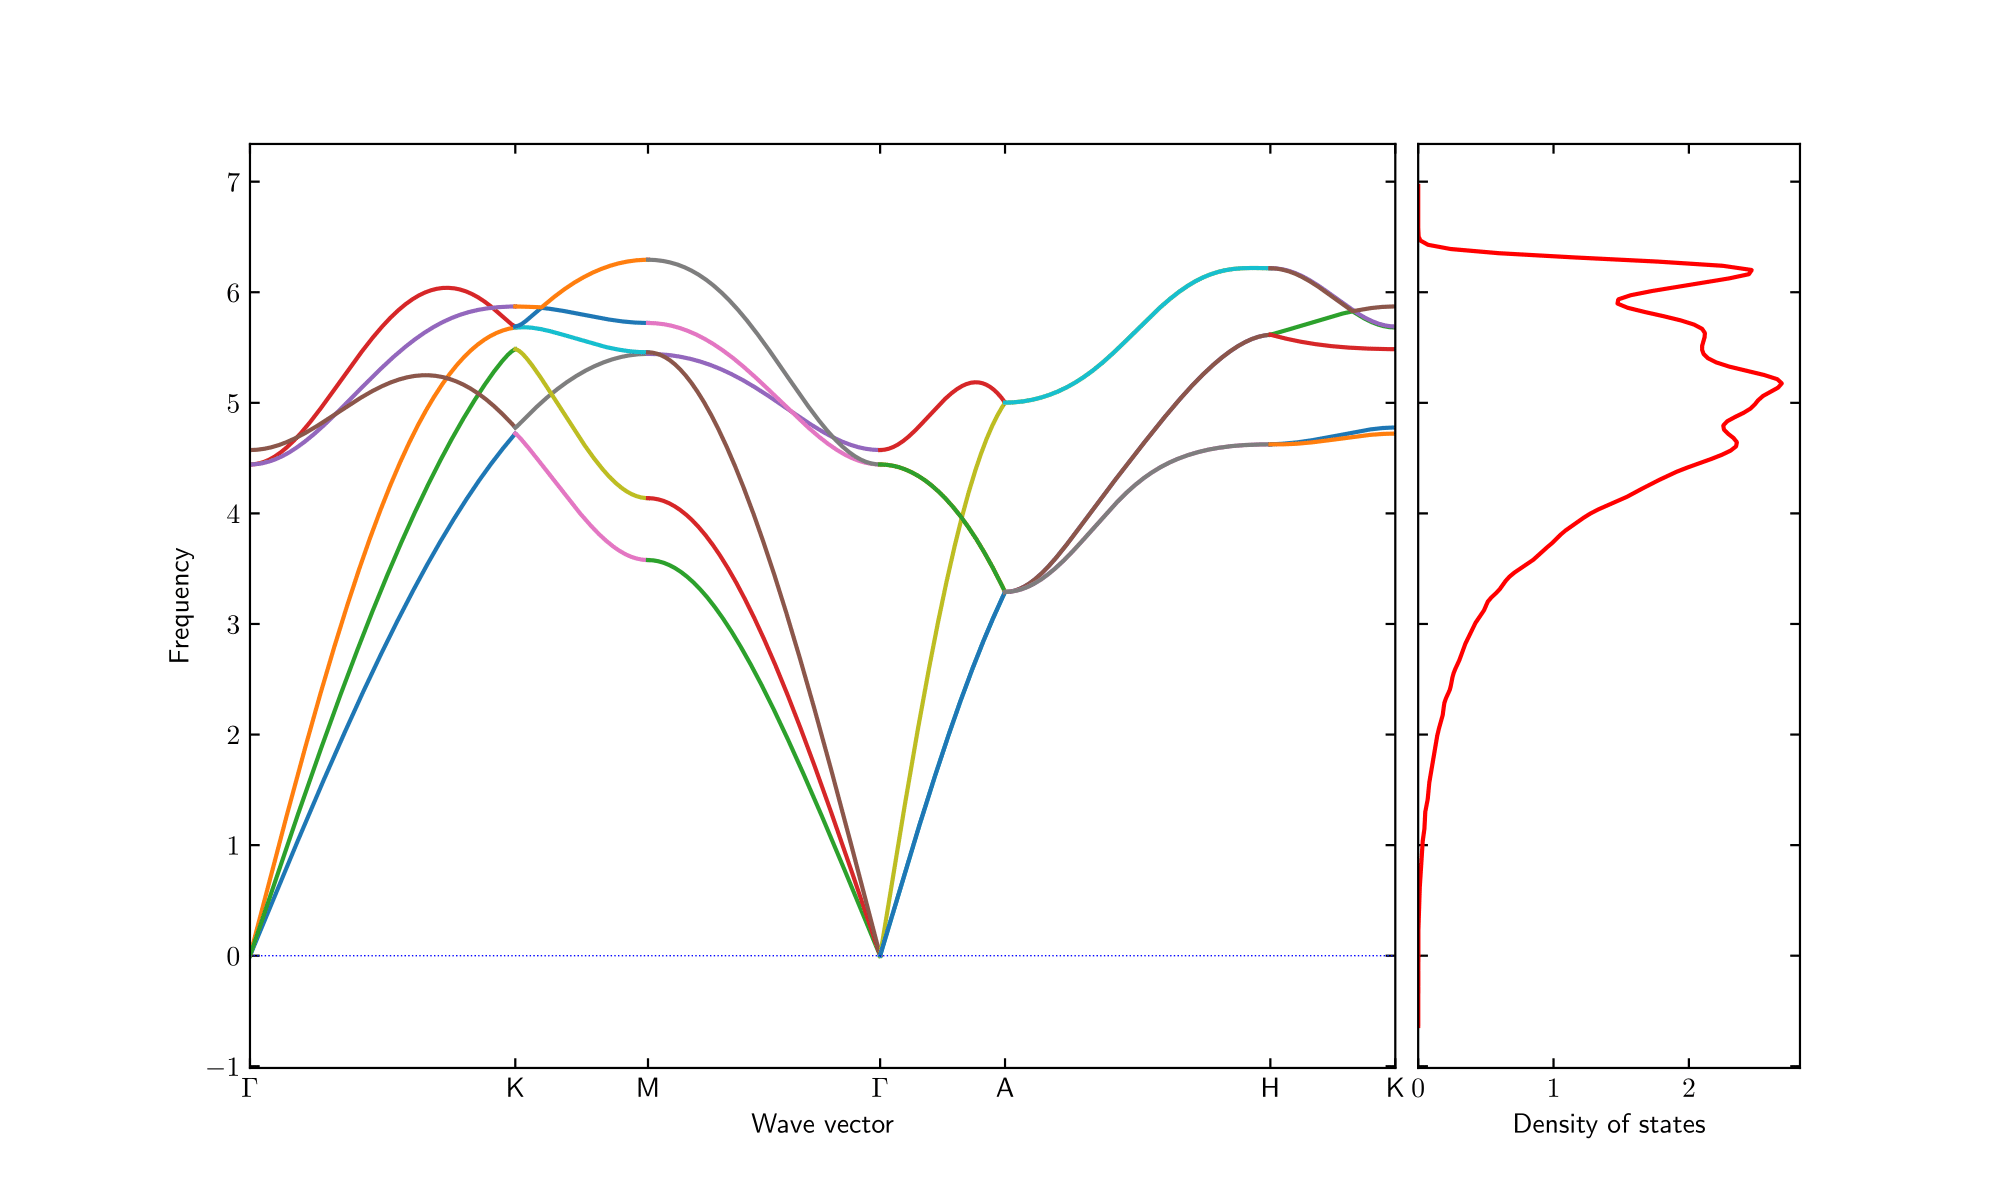
\includegraphics[width=.9\linewidth]{/home/tigany/Documents/docs/Management/Images/hcp-band_dos_2019-03-21-1.png}
\label{org78afb0b}
\end{center}

\begin{center}
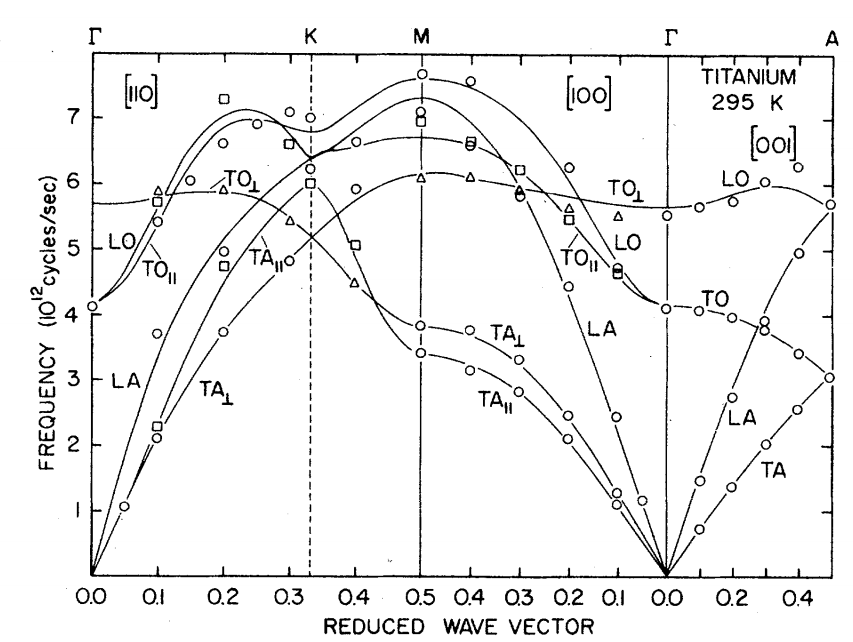
\includegraphics[width=.9\linewidth]{/home/tigany/Documents/docs/Management/Images/experimental_hcp_phonons.png}
\end{center}

\begin{notes}
All frequencies are in THz
\end{notes}

\subsection*{\(\omega\) phase}
\label{sec:org7faa9bd}
\begin{center}
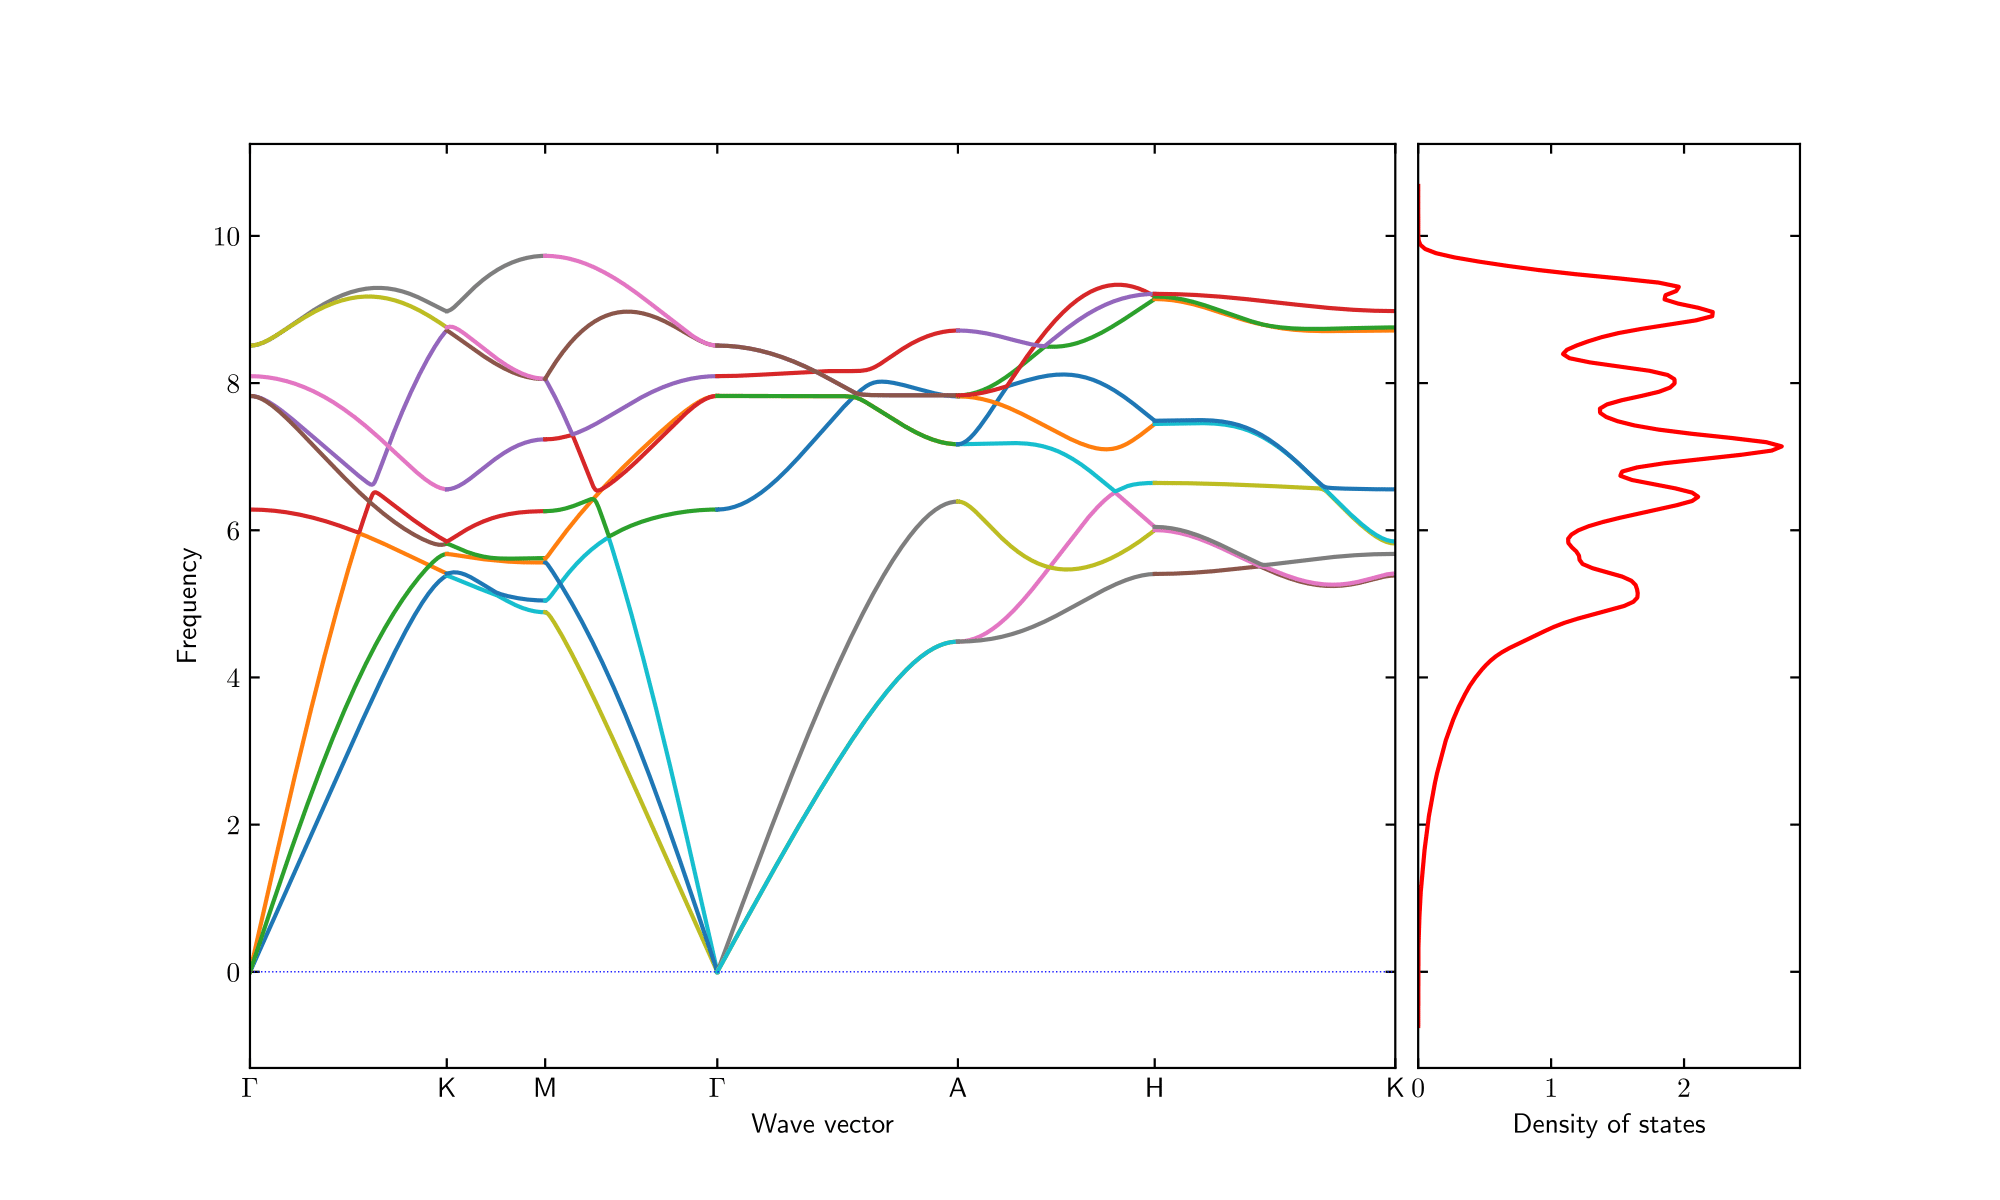
\includegraphics[width=.9\linewidth]{/home/tigany/Documents/docs/Management/Images/omega-band_dos_2019-03-21-1.png}
\label{orge287774}
\end{center}

\begin{center}
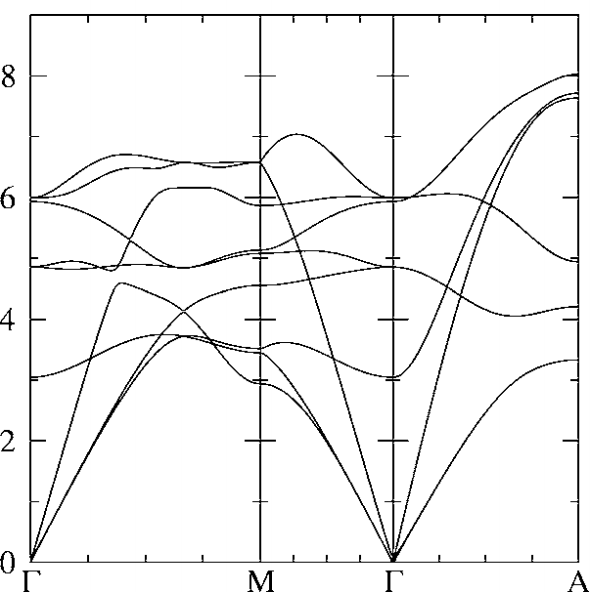
\includegraphics[width=.9\linewidth]{/home/tigany/Documents/docs/Management/Images/omega_phonons_trinkle.png}
\end{center}


\subsection*{\(\beta\) phase}
\label{sec:org986085a}
\begin{center}
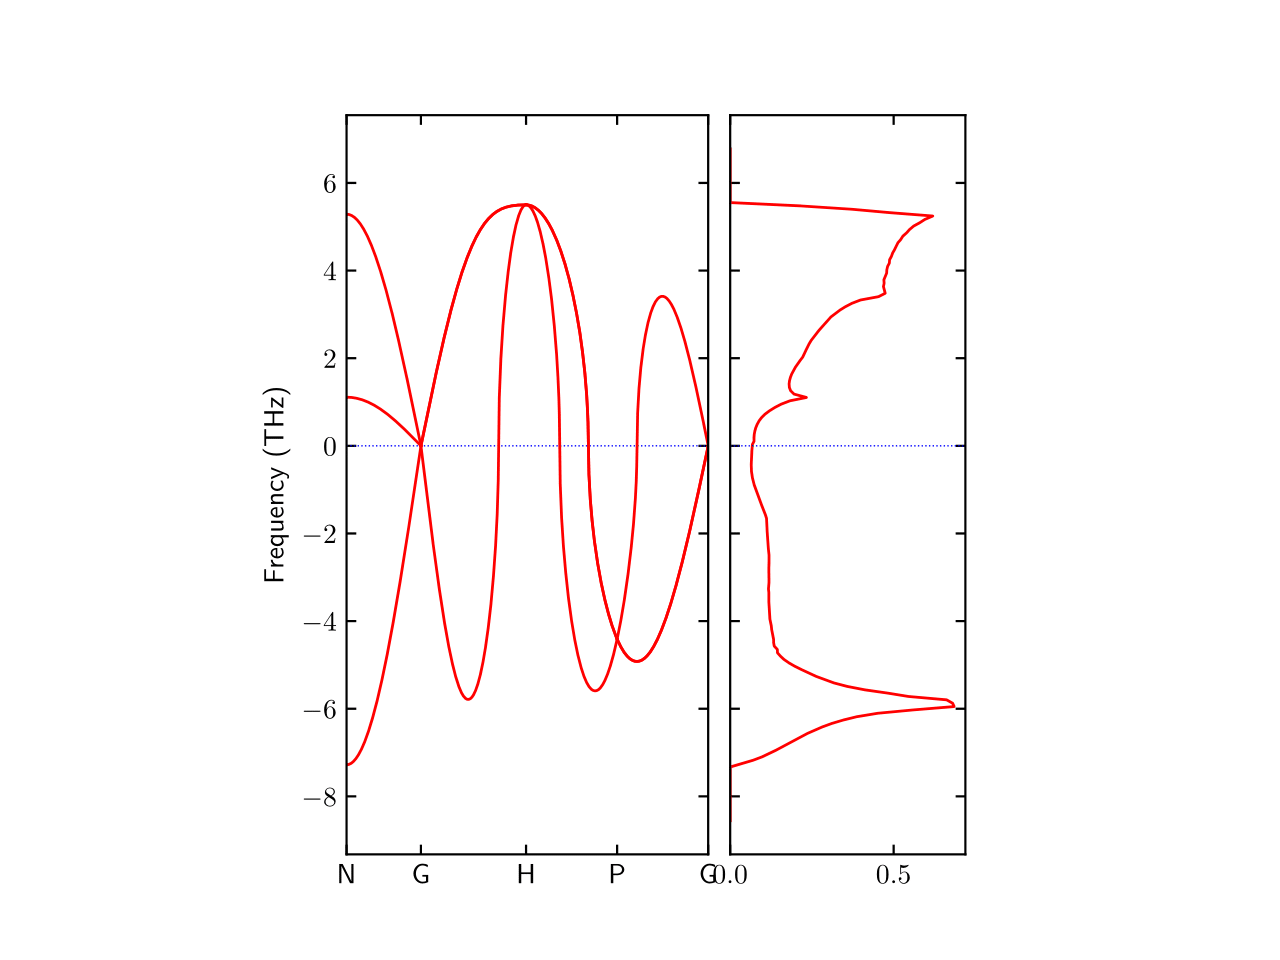
\includegraphics[width=.9\linewidth]{/home/tigany/Documents/docs/Management/Images/bcc-band_dos_rightconf-1.png}
\label{org2dceba5}
\end{center}



\begin{center}
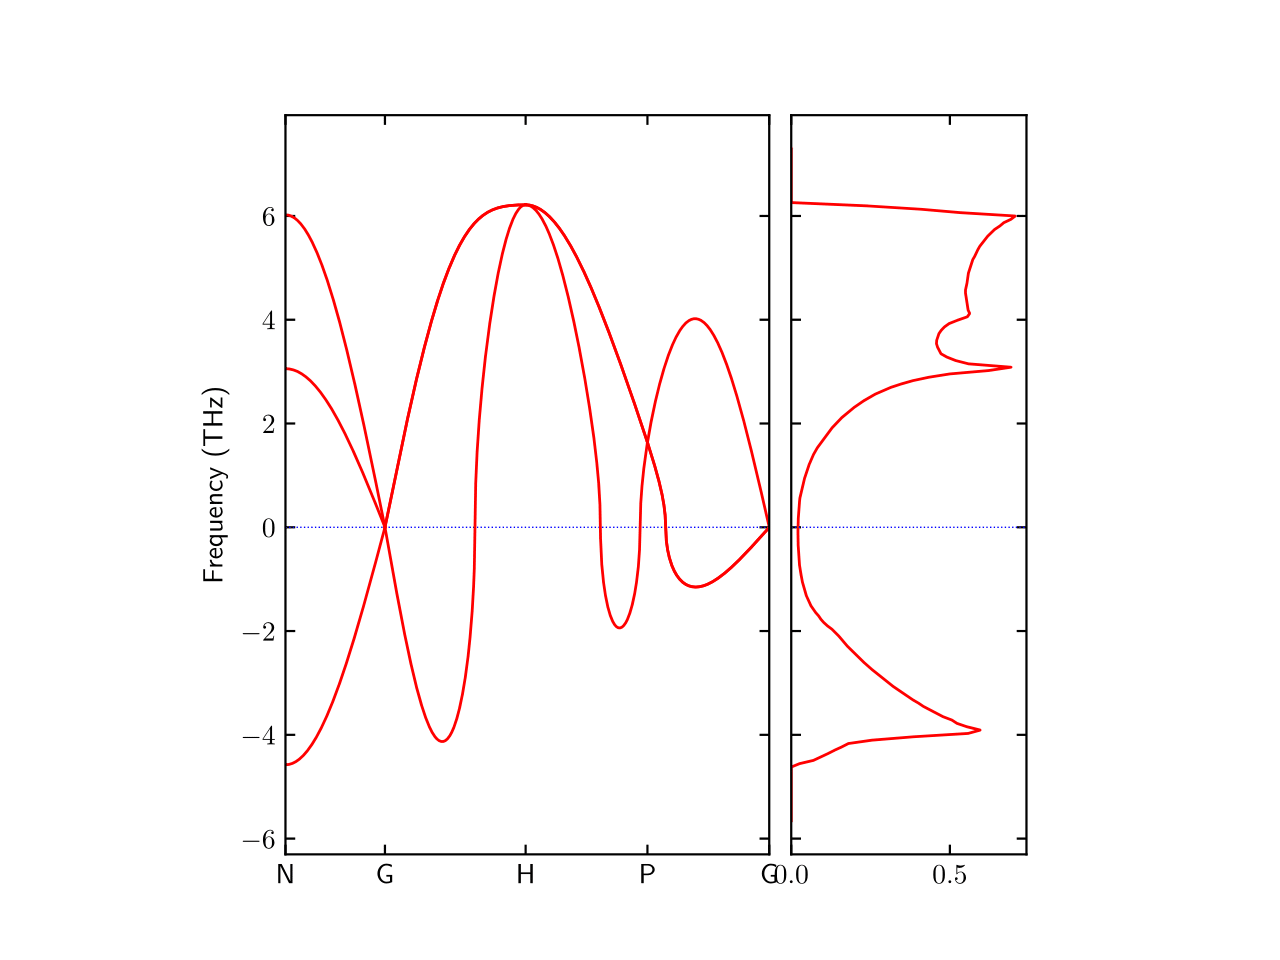
\includegraphics[width=.9\linewidth]{/home/tigany/Documents/docs/Management/Images/bcc-band_dos_dft-1.png}
\end{center}
\section*{Free Energies}
\label{sec:org0aba707}


\subsection*{Vibrational Free Energy}
\label{sec:orgda774f8}
\begin{center}
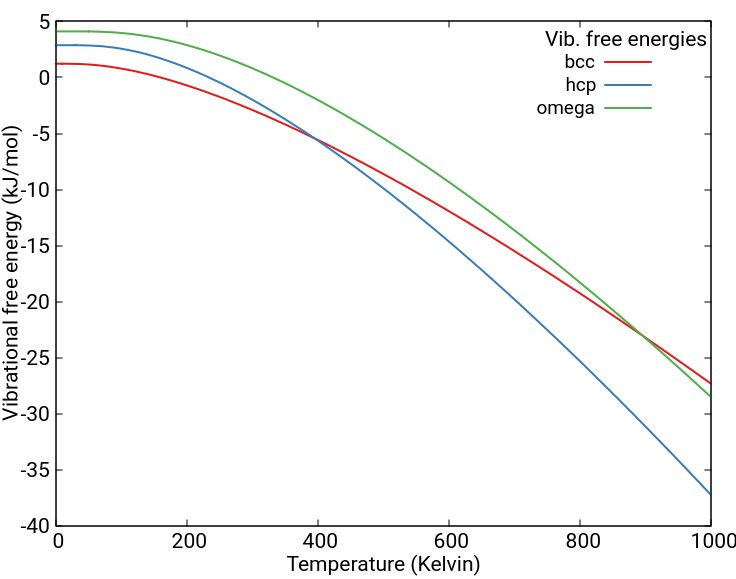
\includegraphics[width=.9\linewidth]{/home/tigany/Documents/docs/Management/Images/vibrational_free_energy_2019-04-04.png}
\label{org18cd2fa}
\end{center}

\begin{center}
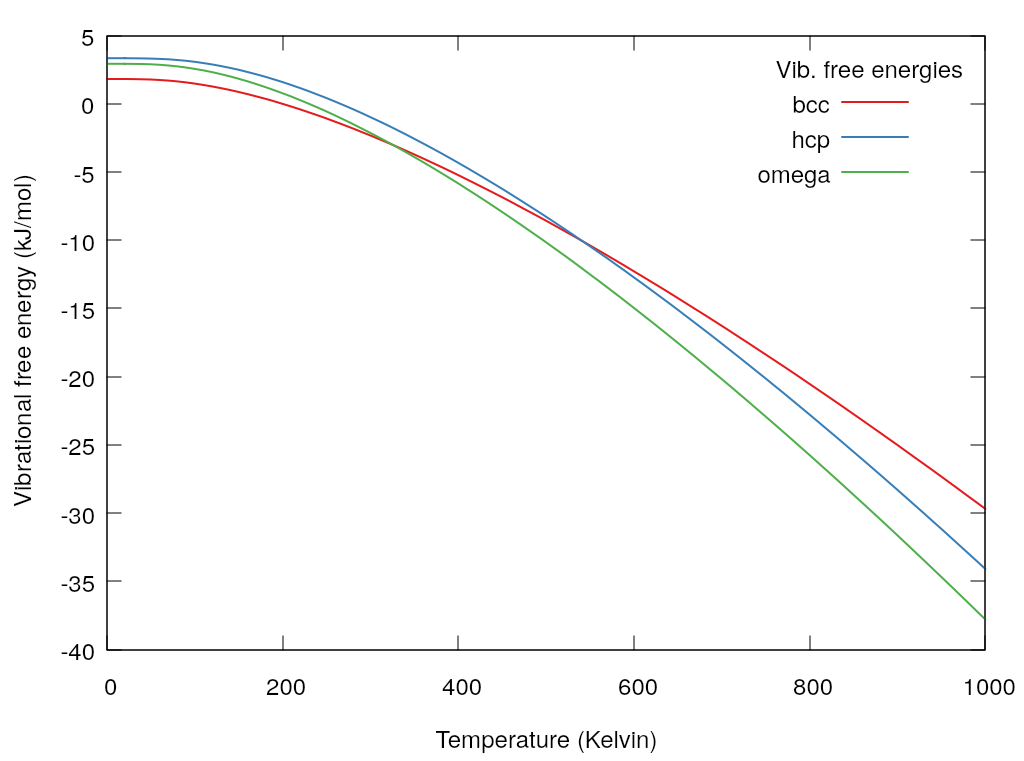
\includegraphics[width=.9\linewidth]{/home/tigany/Documents/docs/Management/Images/vibrational_free_energy_lda.png}
\end{center}

\subsection*{Total Free Energy}
\label{sec:orgf665cf0}
\begin{center}
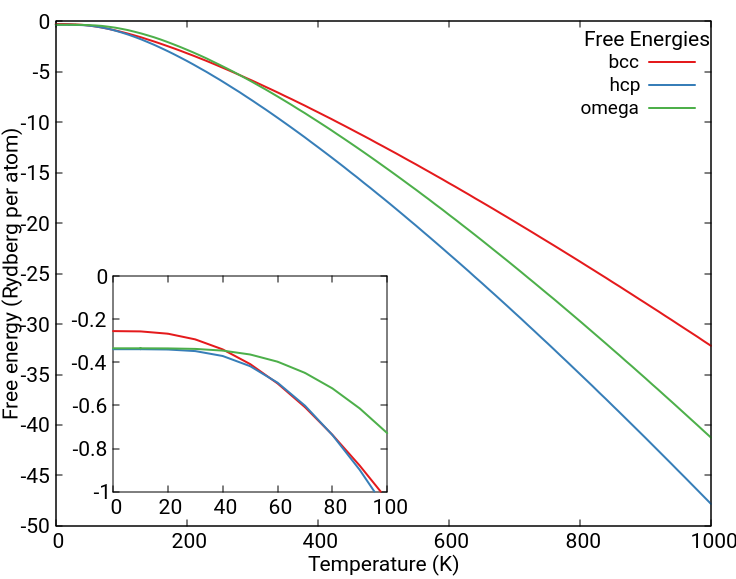
\includegraphics[width=.9\linewidth]{/home/tigany/Documents/docs/Management/Images/enthalpy_and_vibrational_Rydberg_alternate_tbe_thick.png}
\label{orgd46b59b}
\end{center}


\begin{center}
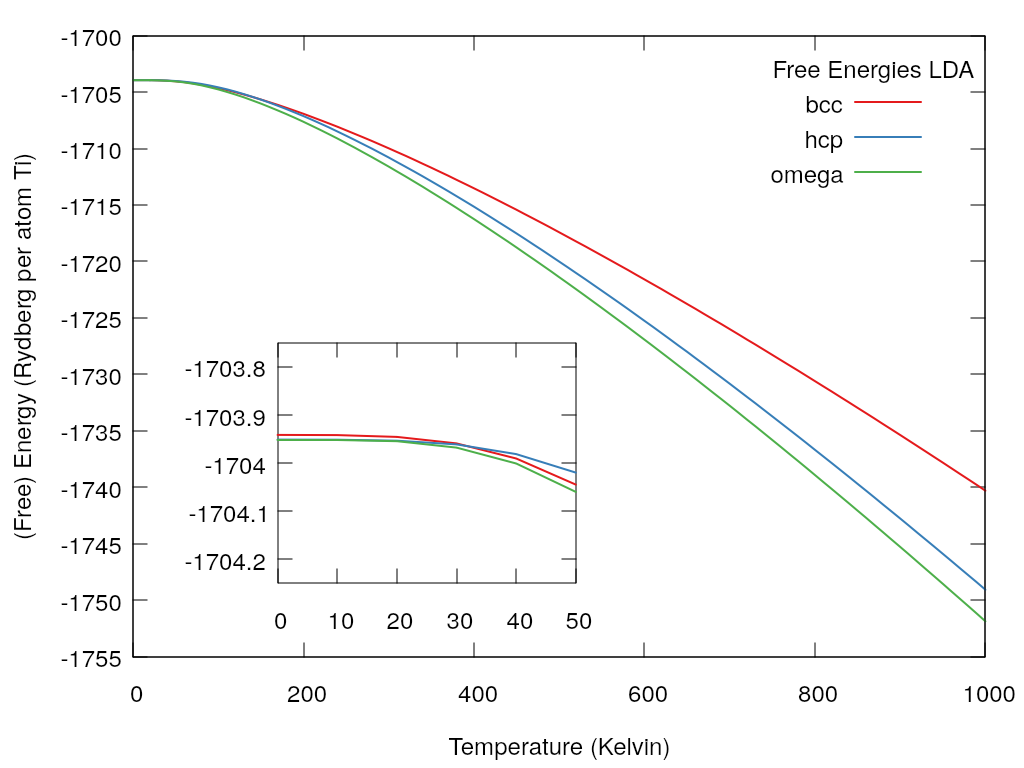
\includegraphics[width=.9\linewidth]{/home/tigany/Documents/docs/Management/Images/enthalpy_and_vibrational_Rydberg_alternate_lda_thick.png}
\end{center}


\begin{NOTES}



Free energy contribution from soft phonon modes don't contribute alot to the
free energy, hence why at the larger temperatures the bcc phase does not
dominate. 

bcc is not favoured and then at around 55-80K it is favoured marginally compared
to the hcp structure. 
After this the hcp structure is favoured with bcc again becoming the one least
favourable. 

hcp is always more stable than omega in this temperature range. 
\end{NOTES}

\section*{Gamma Surfaces}
\label{sec:org0b1eb9f}


\begin{itemize}
\item \(\gamma\) -surfaces are plots of excess energy with the movement of
atoms on a fault plane.
\item Stable stacking faults correspond to local minima.
\item This provides insight into possible dislocation dissociations.
\end{itemize}

\subsection*{Basal gamma surfaces}
\label{sec:org85d07be}


\begin{center}
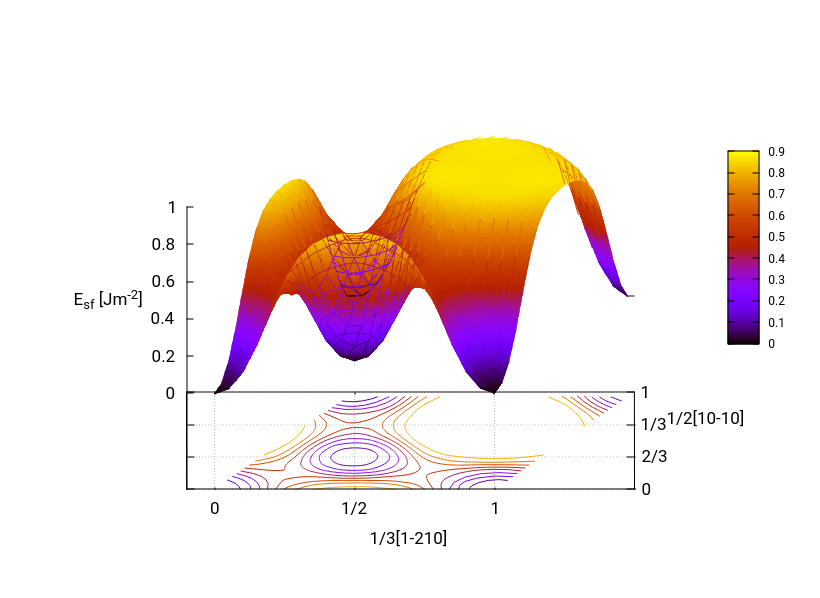
\includegraphics[width=.9\linewidth]{/home/tigany/Documents/docs/Management/Images/basal_gamma_surface_tbe_2019-03-21_format_2.png}
\label{orgc5c8da3}
\end{center}


\begin{center}
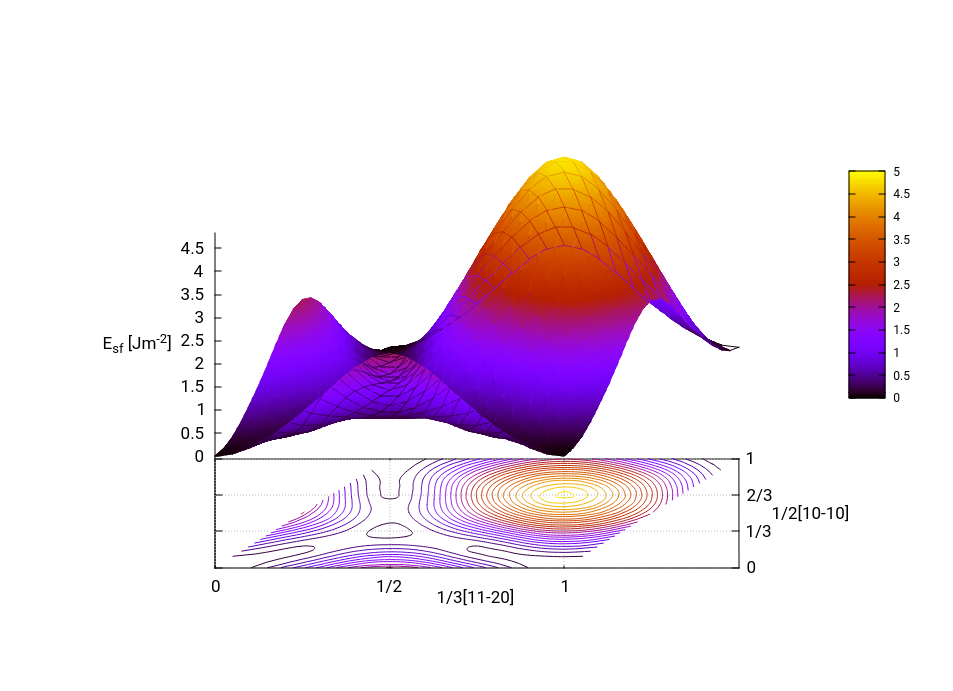
\includegraphics[width=.9\linewidth]{/home/tigany/Documents/docs/Management/Images/basal_gamma_surface_bop_2019-03-30_format_2.png}
\end{center}


\begin{center}
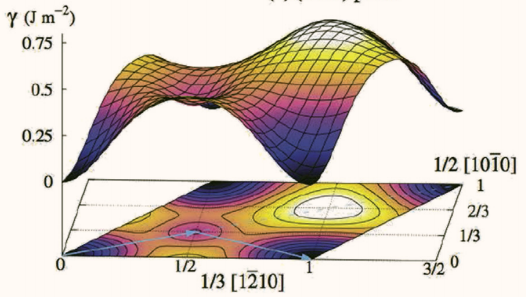
\includegraphics[width=.9\linewidth]{/home/tigany/Documents/docs/Management/Images/rodney_basal_ti_gamma_surface.png}
\end{center}

Expected splitting (all models): \(\frac{1}{3}[1\bar{2}10] = \frac{1}{3}[1\bar{1}00] +  \frac{1}{3}[0\bar{1}10]\)

\subsection*{Prismatic gamma surfaces}
\label{sec:org9d4a1f2}

\begin{center}
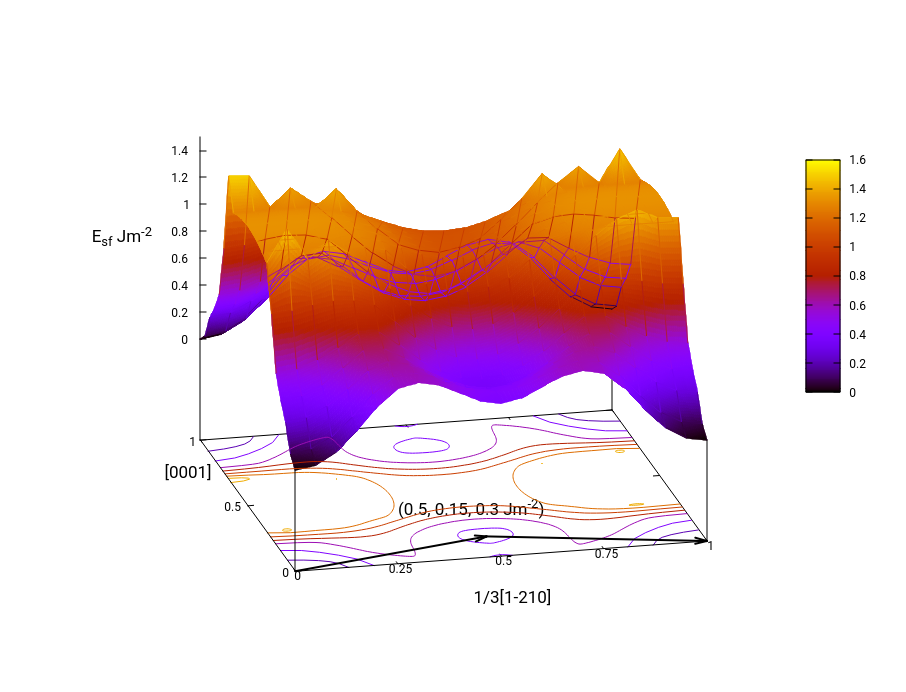
\includegraphics[width=.9\linewidth]{/home/tigany/Documents/docs/Management/Images/prismatic_gamma_surface_2019-12-28_tbe.png}
\end{center}


\begin{center}
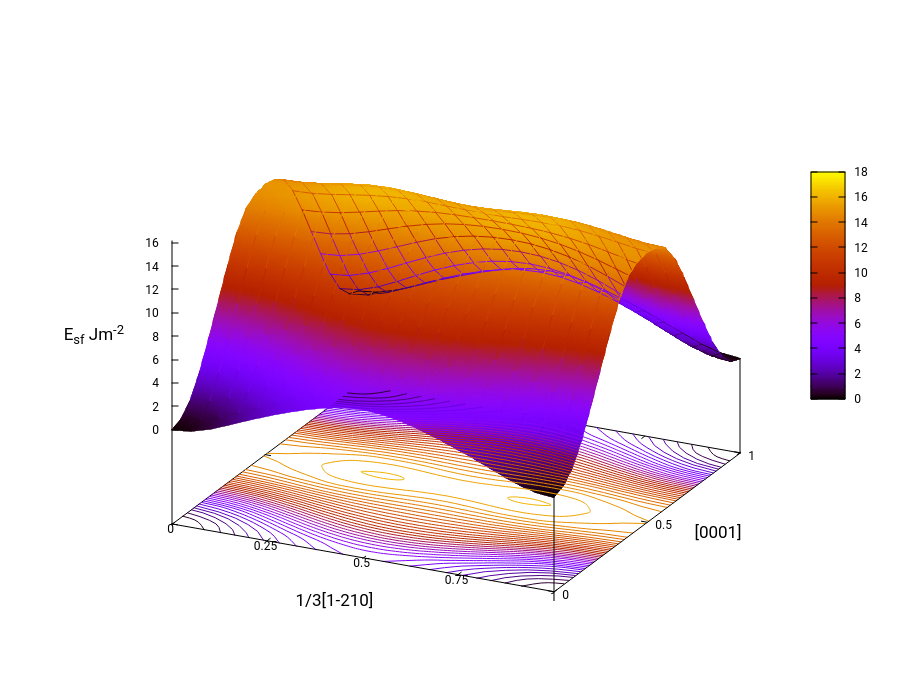
\includegraphics[width=.9\linewidth]{/home/tigany/Documents/docs/Management/Images/prismatic_gamma_surface_2019-12-28_bop.png}
\end{center}



\begin{center}
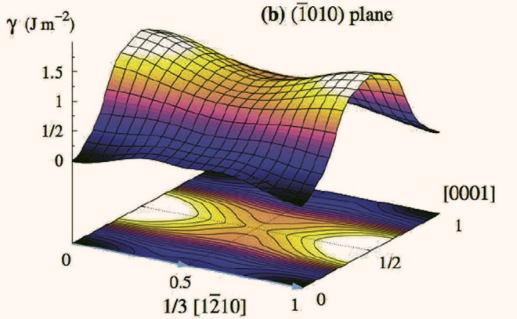
\includegraphics[width=.9\linewidth]{/home/tigany/Documents/docs/Management/Images/rodney_prismatic_ti_gamma_surface.png}
\end{center}


\begin{itemize}
\item Theoretical splitting: \(\frac{1}{3}[1\bar{2}10] = \frac{1}{6}[1\bar{2}10] + \frac{1}{6}[1\bar{2}10]\)
\item Expected splitting (TB): \(\frac{1}{3}[1\bar{2}10] = ( \frac{1}{6}[1\bar{2}10] + 0.15[0001]) + ( \frac{1}{6}[1\bar{2}10] - 0.15[0001] )\)
\item Expected splitting (BOP): None.
\end{itemize}

\begin{NOTES}


From TB one can see that the splitting is immediately not exactly the same as
that of DFT. 
\end{NOTES}

\subsection*{Pyramidal gamma surfaces}
\label{sec:orge09ef90}
\begin{center}
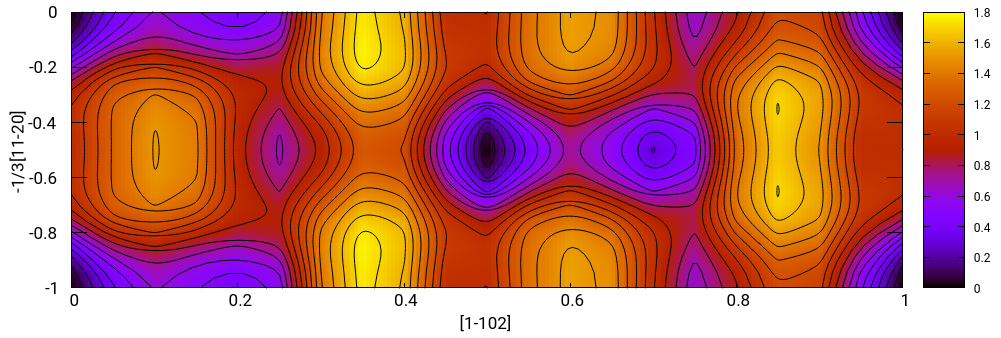
\includegraphics[width=.9\linewidth]{/home/tigany/Documents/docs/Management/Images/pyramidal_gamma_surface_2019-03-27_mapped.png}
\label{org2f7bef7}
\end{center}

\begin{notes}


One can see a saddle point in the interatomic potential and the tb model. So
one can assume that this is a point which relies on subtle electronic
structure methods. Like the prismatic splitting above. 
\end{notes}

\subsection*{Results}
\label{sec:org0aa53a4}
\begin{center}
\begin{tabular}{lllrllll}
 & Plane & Fault & TB & BOP & [DFT] & [TB] & [BOP]\\
\hline
 & Basal & \(I_{2}\) & 19 & 127 & 260 \(^{[1]}\) & 290 \(^{[2]}\) & 110 \(^{[3]}\)\\
\hline
 & Prismatic & \(\gamma_{P}\) & 299 & 4618 & 250/233 \(^{[1,4]}\) & 110\(^{[5]}\) & 260\(^{[3]}\)\\
\hline
 & Pyramidal & \(I_{1}\) & 288 & -- & 288 \(^{[6]}\) & -- & --\\
 &  & \(I_{2}\) & 671 & -- & 788 \(^{[6]}\) & -- & --\\
\end{tabular}
\end{center}


\begin{itemize}
\item Units are in \(mJm^{-2}\). Square brackets denote method from literature.
\item \(^{[1]}\) Benoit (2012), \(^{[2]}\) Bere (1999), \(^{[3]}\) Girshick (1998)
\item \(^{[4]}\) Ackland (1992), \(^{[5]}\) Legrand (1984), \(^{[6]}\) Ready (2019), \(^{[7]}\) Chaari (2014)
\end{itemize}


\begin{NOTES}
Pyramidal plane large minima at 0.5, 0.5, 0.0. 

For I\textsubscript{1} fault I get 288
For the other fault, I get 671 mJm\textsuperscript{-2}

Smaller minima is at 0.7, 0.5, 288 mJm\textsuperscript{-2}

In pseudopotential one gets 288 as well! 


Pair potential for the BOP on fitting needs to be tweaked for accurate
results.
\end{NOTES}


\section*{Core structures}
\label{sec:org41cfd14}
\begin{itemize}
\item Dislocation cores are sensitive to boundary conditions.
\item Sufficient resolution of core structure is necessary ascertain how
dislocation glide is modified.
\end{itemize}



\subsection*{Quadrupolar Cell \(\frac{1}{3}\langle11\bar{2}0\rangle\) screw}
\label{sec:org13d9eb3}


\url{file:///home/tigany/Documents/docs/Management/Images/core\_relax\_initial.gif}
\begin{center}
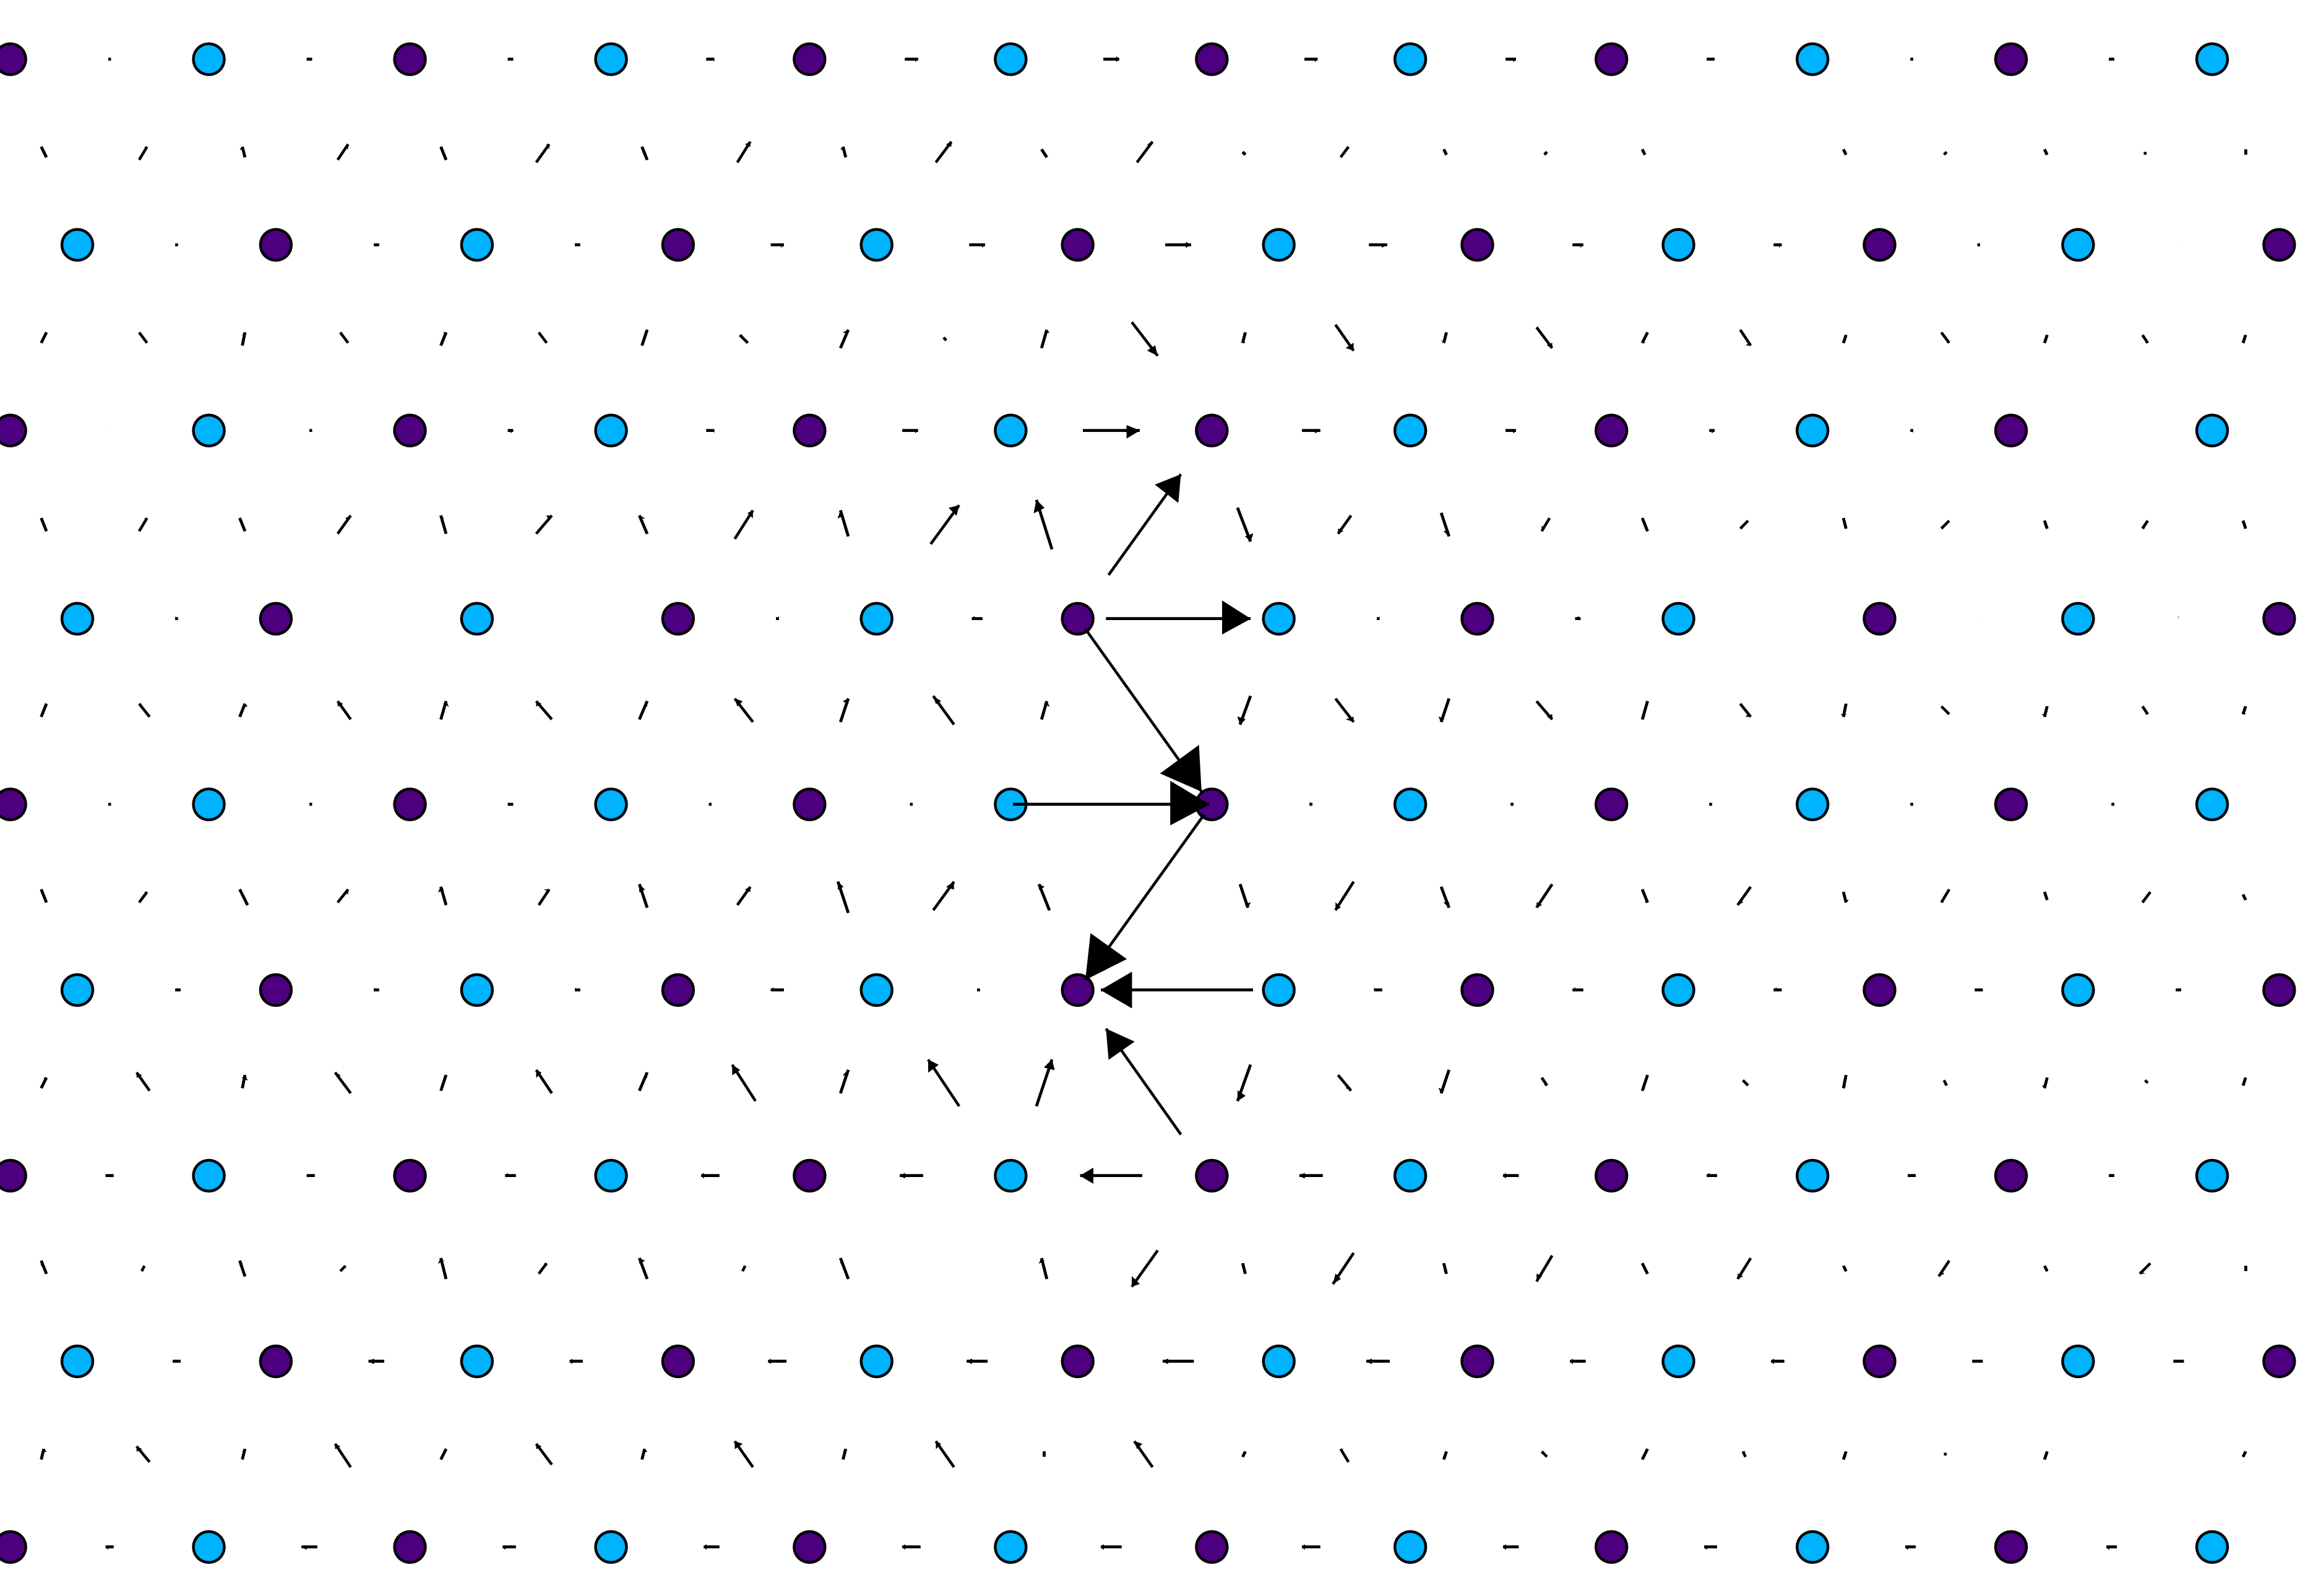
\includegraphics[width=.9\linewidth]{/home/tigany/Documents/docs/Management/Images/zoom_core_look.png}
\end{center}

\begin{center}
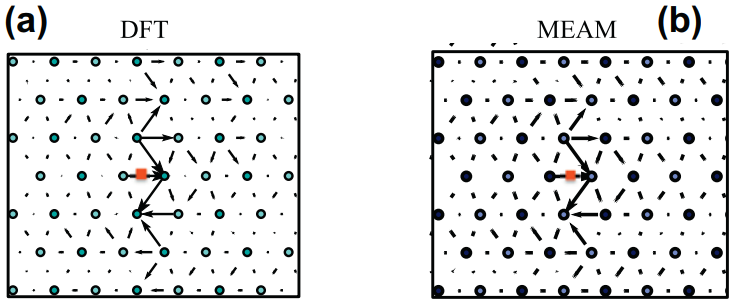
\includegraphics[width=.9\linewidth]{/home/tigany/Documents/docs/Management/Images/ghazisaiedi_trinkle_3_core.png}
\end{center}

\begin{center}
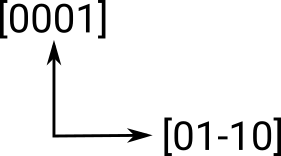
\includegraphics[width=.9\linewidth]{/home/tigany/Documents/docs/Management/Images/coordinate_prismatic_plane.png}
\end{center}


\subsection*{Oxygen-core quadrupole}
\label{sec:org8b5287b}



\section*{Vacancy formation energy}
\label{sec:orgd87dcd5}

\begin{center}
\begin{tabular}{lr}
\(\Delta E_{\text{f}}^{\text{vacancy}}\) & [eV]\\
\hline
Relaxed & 1.01\\
(Exp.) Hashimoto (1984) & 1.27\\
(DFT) GGA-PAW: Angsten (2013) & 1.95\\
\hline
\end{tabular}
\end{center}



\section*{Molecular Dynamics}
\label{sec:org747a238}



\section*{Future Work}
\label{sec:org3ab9656}
\begin{itemize}
\item Obtain a model of Ti that more closely matches empirical quantities.
\item See how core structure changes with O content.
\item Calculate the Peierls barrier on prism, and \(\pi\) planes.
\item Calculate secondary Peierls barrier for kink migration with and without
oxygen.
\item Add rutile layer; see how dislocations and oxygen interact with structure.
\end{itemize}


\section*{Additional references}
\label{sec:org281f56c}

\begin{itemize}
\item Ghazisaeidi, Trinkle (2012), \emph{Core structure of a screw dislocation in Ti from density functional theory and classical potentials}.
\item Rodney, Ventelon (2016), \emph{Ab initio modelling of dislocation core properties
in metals and semiconductors}.
\item Chaari, Clouet (2014), \emph{First order pyramidal slip of 1/3 screw dislocations in zirconium}
\end{itemize}
\end{document}
